\documentclass[11pt]{article}
\usepackage{../../Utility/Template}
\usepackage[raggedright]{titlesec}
\setcounter{secnumdepth}{5}
\setcounter{tocdepth}{5}
\usepackage{hyperref}
\usepackage{listings}
\usepackage{pdflscape}
\usepackage{enumitem}
\usepackage{afterpage}
\usepackage{float}

\setlength{\abovecaptionskip}{0pt plus 3pt minus 2pt}

\titleformat{\paragraph}[hang]{\normalfont\normalsize\bfseries}{\theparagraph}{1em}{}
\titlespacing*{\paragraph}{0pt}{3.25ex plus 1ex minus .2ex}{0.5em}
 
\definecolor{coloreRossoChiaro}{HTML}{934037}

\usepackage{listings}
\usepackage{float}

\definecolor{backcolour}{rgb}{0.95,0.95,0.92}

\lstdefinelanguage{JavaScript}{
  keywords={typeof, new, true, false, catch, function, return, null, catch, switch, var, if, in, while, do, else, case, break, it, describe, AuthenticationService, beforeEach, spyOn, try},
  keywordstyle=\color{blue}\bfseries,
  ndkeywords={class, export, boolean, throw, implements, import, this, async, await},
  ndkeywordstyle=\color{red}\bfseries,
  identifierstyle=\color{black},
  sensitive=false,
  comment=[l]{//},
  morecomment=[s]{/*}{*/},
  commentstyle=\color{purple}\ttfamily,
  stringstyle=\color{blue!50}\ttfamily,
  morestring=[b]',
  morestring=[b]"
}

\renewcommand{\lstlistingname}{Esempio di codice}

\lstdefinestyle{mystyle}{
    backgroundcolor=\color{backcolour},   
    %commentstyle=\color{green},
    keywordstyle=\color{red},
    %numberstyle=\tiny\color{blue},
    %stringstyle=\color{blue!50},
    basicstyle=\ttfamily\footnotesize,
    breakatwhitespace=false,         
    breaklines=true,                 
    captionpos=b,                    
    keepspaces=true,                 
    numbers=left,                    
    numbersep=5pt,                  
    showspaces=false,                
    showstringspaces=false,
    showtabs=false,                  
    tabsize=2
}

\lstset{style=mystyle}

\begin{document}
\newcommand{\Titolo}{Allegato Tecnico}

\newcommand{\Redattori}{\RA{} \newline	\ZM{} \newline \PA{}}

\newcommand{\Verificatori}{\SG{} \newline \BM{}}

\newcommand{\Approvatore}{\SP{}}

\newcommand{\Distribuzione}{\Proponente{} \newline \VT{} \newline \CR{} \newline Gruppo \Gruppo{}}

\newcommand{\Uso}{Interno}

\newcommand{\DescrizioneDoc}{Questo documento racchiude tutte le informazioni necessarie per l'estensione e la manutenzione del prodotto \textit{NFT Lab}.}

\newcommand{\pathimg}{../../Utility/Images/logo2.png}

\newcommand{\Versionedoc}{2.0.0-1.8}
% info generali 

\newcommand{\NomeProgetto}{\textit{NFT Lab}}

% fornitore
\newcommand{\Gruppo}{\textit{CodeBusters}}
\newcommand{\Mail}{codebusterswe@gmail.com}

% committenti
\newcommand{\Committente}{\VT \newline \CR}
\newcommand{\VT}{Prof. Vardanega Tullio}
\newcommand{\CR}{Prof. Cardin Riccardo}

% proponenti
\newcommand{\Proponente}{\textit{Zucchetti}}

% codebusters
\newcommand{\SG}{Sassaro Giacomo}
\newcommand{\BM}{Baldisseri Michele}
\newcommand{\ZM}{Zenere Marco}
\newcommand{\PA}{Pirolo Alessandro}
\newcommand{\SP}{Scialpi Paolo}
\newcommand{\SH}{Safdari Hossain}
\newcommand{\RA}{Rago Alessandro}

% ruoli
\newcommand{\Responsabile}{Responsabile di Progetto}
\newcommand{\Amministratore}{Amministratore di Progetto}

% documenti

\newcommand{\SdF}{\textit{Studio di Fattibilità}}
\newcommand{\SdFv}[1]{\textit{Studio di Fattibilità {#1}}}
\newcommand{\PdQ}{\textit{Piano di Qualifica}}
\newcommand{\PdQv}[1]{\textit{Piano di Qualifica {#1}}}
\newcommand{\PdP}{\textit{Piano di Progetto}}
\newcommand{\PdPv}[1]{\textit{Piano di Progetto {#1}}}
\newcommand{\NdP}{\textit{Norme di Progetto}}
\newcommand{\NdPv}[1]{\textit{Norme di Progetto {#1}}}
\newcommand{\AdR}{\textit{Analisi dei Requisiti}}
\newcommand{\AdRv}[1]{\textit{Analisi dei Requisiti {#1}}}
\newcommand{\Glossario}{\textit{Glossario}}
\newcommand{\Glossariov}[1]{\textit{Glossario {#1}}}
\newcommand{\MM}{\textit{Manuale Manutentore}}
\newcommand{\MMv}[1]{\textit{Manuale Manutentore {#1}}}
\newcommand{\MU}{\textit{Manuale Utente}}
\newcommand{\MUv}[1]{\textit{Manuale Utente {#1}}}

% comandi generali
\newcommand{\glo}[1]{#1\ap{G}}
%\newcommand{\glo}[1]{\textsc{#1\textsuperscript{\textit{G}}}}

\setlength{\parindent}{-0.1em}
\frontespizio 
\fancydoc
%\newpage	
%\input{Section/RegistroModifiche.tex}
\newpage
\tableofcontents
\newpage


\section{Organizzazione del progetto}
Nella directory principale del progetto sono presenti tutti i file di configurazione degli strumenti utilizzati, come le impostazioni dell'IDE, la configurazione della continuos integration e i file per il versionamento attraverso Git. Oltre a questo, è presente la cartella \textbf{\textit{src}} al cui interno si trovano i file del prodotto vero e proprio. La struttura è organizzata nel seguente modo:
\begin{itemize}
    \item[--] \textbf{File principali}: \textit{index.html}, \textit{styles.css} e \textit{main.ts}, utilizzati a livello globale dalla web app;
    
    \item[--] \textbf{Cartella \textit{environments}}: contiene le variabili globali, sia per il prodotto in fase di sviluppo sia nel momento in cui entra in produzione (per esempio sono presenti le variabili utili per modificare le chiamate API); 
    
    \item[--] \textbf{Cartella \textit{e2e}}: contiene gli script dei test \textit{end to end} creati con Taiko;
    
    \item[--] \textbf{Cartella \textit{assets}}: è accessibile da qualsiasi file e contiene tutte le risorse che la web application utilizza, come immagini o documenti. Inoltre qualsiasi risorsa contenuta è raggiungibile via browser tramite richiesta HTTP;
    
    \item[--] \textbf{Cartella \textit{app}}: comprende a sua volta il contenuto riportato di seguito.
    
        \begin{itemize}
            \item \textbf{Cartella \textit{mocks}}: contiene file utili in fase di test per creare un \textit{mock} di componenti o servizi;
            
            \item \textbf{Cartella \textit{models}}: contiene le interfacce degli oggetti che rappresentano il dominio del progetto;
            
            \item \textbf{Cartella \textit{services}}: contiene tutti i servizi utilizzati dai componenti per effettuare le chiamate API;
            
            \item \textbf{Cartella \textit{shared}}: contiene tutti i componenti che sono stati riutilizzati.
            
            \item Una cartella \textbf{per ogni pagina} del sito, che comprende tutti i componenti utilizzati in ciascuna.
        \end{itemize}
\end{itemize}

\section{Continuous integration}
Sul repository di progetto è stato creato un workflow che viene attivato automaticamente ad ogni push. Questo permette di:
\begin{itemize}
\item Installare le dipendenze tramite \textit{Node Package Manager};
\item Eseguire il processo di \textit{build} dell’applicazione;
\item Eseguire i test d’unità e calcolare la code coverage;
\item Caricare i risultati dei test su \textit{Coveralls}.
\end{itemize}
Il workflow in questione può essere modificato per estenderne le funzionalità o per collegare il repository ad altri servizi esterni.

\section{Servizi}
In questa sezione vengono riportati tutti i servizi creati, il loro compito e i componenti che utilizzano questa dipendenza.

\begin{itemize}
    \item \textbf{AuthenticationService}: presenta il metodo per effettuare l'autenticazione dell'utente nel sistema. Se le informazioni, e-mail e password, sono corrette e individuano un'istanza nel database, viene ritornato un JSON contenente tutte le informazioni dell'utente, in modo da salvarle nel \textit{local storage}. Il componente che dipende da questo servizio è \textit{login-form-component}.
    
    \begin{lstlisting}[language=JavaScript, numbers=none, caption=Esempio di JSON ritornato dal servizio di autenticazione]
    
    //user informations
    {
        id: 12,
        name: "test",
        surname: "test",
        email: "test06@gmail.com",
        dob: "1998-06-01",
        wallet: "0xEd1bB395f00B22454c22B6c76b645657c739D3cc",
        age: 23
    }
    \end{lstlisting}
    
    \item \textbf{CategoriesService}: presenta il metodo per richiedere tutte le tipologie di categorie presenti nel database. I componenti che dipendono da questo servizio sono \textit{filter-search}, \textit{modify-opera-form}, \textit{new-opera-form} ed \textit{opera-management}.
    
    \begin{lstlisting}[language=JavaScript,numbers=none, caption=Esempio di JSON ritornato dal servizio di richiesta delle categorie]
    
    //categories
    {
        [
            {id: 1, name: "food"}, {id:2, name: "sport"}
        ]
    }
    
    \end{lstlisting}
    
    \item \textbf{OperaManagementService}: presenta tutti i metodi che riguardano la gestione delle opere dell'utente, quali le richiesta di tutte le sue opere, la modifica di un'opera e l'aggiunta di una di nuova. I componenti che dipendono da questo servizio sono \textit{modify-opera-form}, \textit{new-opera-form} ed \textit{opera-management}.
    
    \newpage
    
    \item \textbf{OperasService}: presenta il metodo per richiedere tutte le opere in vendita. Il componente che dipende da questo servizio è \textit{home}.
    
    \begin{lstlisting}[language=JavaScript, numbers=none, caption=Esempio di JSON utilizzato per le opere]
    
    //opera informations
    {
        id:"Qmb13ALEkqXtV5DT6jcrXuUGjat",
        title: "test",
        description: "test",
        authorId: 18,
        price: 52.0,
        currency: "ETH",
        status: false,
        path: "gallery/Qmb13ALEkqXtV5DT6jcrXuUGjat.jpg",
        type: "img",
        owner: "test",
        author: "test",
        categories: [{id: 2, name:"sport"}]
    }
    
    \end{lstlisting}
    
    \item \textbf{SignupService}: presenta il metodo per inviare la richiesta di registrazione dell'utente nel sistema. Il componente che dipende da questo servizio è \textit{signup-form}.
    
    \item \textbf{UserManagementService}: presenta tutti i metodi che riguardano la gestione delle informazioni dell'utente, quali la modifica dei suoi dati e la modifica della password per accedere al sistema. I componenti che dipendono da questo servizio sono \textit{modify-user-form} e \textit{modify-psw-form}.
    
    \begin{lstlisting}[language=JavaScript, numbers=none, caption=Esempio di JSON utilizzato per la richiesta di modifica password]

    {
        oldPassword: "Test123@",
        newPassword: "Test123@123"
        email: "test@test.com"
    }
    
    \end{lstlisting}
    
\end{itemize}


\section{Implementazione}
Per lo sviluppo dell'interfaccia grafica si è deciso di utilizzare la libreria \textit{Angular Material}, per sfruttare componenti con proprio stile, e \textit{Flex Layout}, per rendere il sito responsive e diminuire le righe di codice dei file CSS. Nel file \textit{app.module.ts} sono importati solamente i moduli di Angular Material che sono stati effettivamente utilizzati; per una maggiore leggibilità i moduli sono contenuti all'interno dell'array \textit{materialModules}.

\newpage

\begin{figure}[!htb]
\centering
	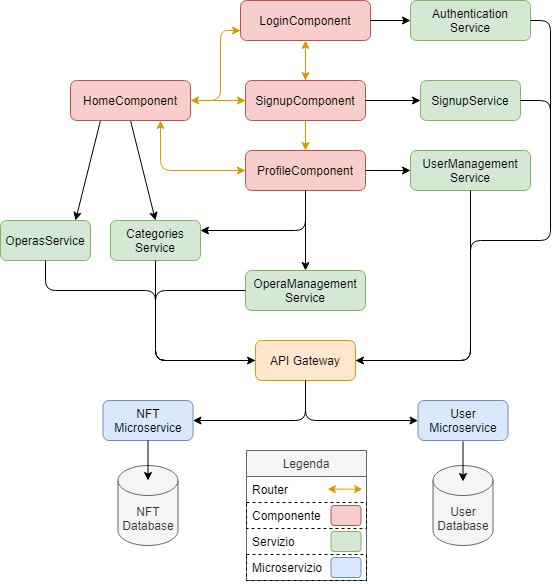
\includegraphics[width=17cm]{Images/progettazione}
	\caption{Componenti dell'applicativo e relativi collegamenti}
\end{figure}


La figura fa notare come l’applicativo sia sviluppato su cinque livelli. Al primo livello troviamo i componenti Angular con il compito di visualizzare e gestire i dati. I service stanno al secondo livello, e forniscono la gestione delle chiamate HTTP al back-end tramite l’API Gateway che, in base alla richiesta ricevuta dal service, chiama il microservizio dedicato a rispondere. In ultimo livello troviamo il database sul quale effettuare le operazioni richieste.

\newpage

\subsection{Registrazione e autenticazione dell'utente}

La pagina di registrazione si presenta con un semplice form per la compilazione di tutti i campi (nonché FormControl soggetti a validazione) necessari all'inserimento dell'utente nel sistema. Al momento della conferma, nel caso in cui l'utente non compilasse correttamente il form, verranno presentati dei messaggi d'errore esplicativi, in modo da guidarlo durante questa fase. Se tutti i dati inseriti sono corretti viene richiamato \textit{SignupService}, il quale effettuerà la POST. Se la risposta avrà esito positivo l'utente verrà reindirizzato nella \textit{home}, altrimenti verrà visualizzato un errore in base all' \textit{HTTP status code} ottenuto.\\
\\
\textbf{Esempio di password valida}: Test123@\\
\textbf{Esempio di un indirizzo di wallet valido}: 0xEd1bB395f00B22454c22B6c76b645657c739D3cc\\
\\
La pagina di autenticazione è molto simile (ma più semplice) e presenta le stesse caratteristiche della pagina precedente. In questo caso verrà chiamato \textit{AuthenticationService}, che effettuerà la POST per recuperare le informazioni dell'utente. Queste vengono poi salvate nel \textit{local storage}, in modo da poterle utilizzare dove necessario.

\subsection{Pagina di profilo dell'utente}
In questa pagina sono presenti sia le informazioni dell'utente che la parte di gestione delle opere in suo possesso. Tutti i pulsanti presenti in questa pagina apriranno un modale dedicato.\\
Per quanto riguarda la prima parte, le informazioni visualizzate vengono prelevate dal \textit{local storage}, presenti in seguito al login. L'utente può inoltre cliccare sul proprio indirizzo del wallet per essere reindirizzato sul sito \textit{www.blockchain.com} ed avere così ulteriori informazioni sullo stato del proprio conto. Al di sotto sono visibili i pulsanti di modifica dei propri dati: anche in questo caso, entrambi i modali, presentano delle form soggette a validazione del contenuto inserito e l'utente sarà sempre avvisato in caso d'errore. Nonostante la modifica della password sia gestita separatamente rispetto agli altri dati, viene richiamato lo stesso servizio, \textit{UserManagementService}, che si occupa di gestire entrambe le PUT. In caso di esito positivo, i dati presenti nel \textit{local storage} verranno aggiornati; questa operazione non sarà effettuata per la modifica della password perché, essendo dato privato e sensibile, non può essere salvato localmente.\\
La seconda sezione è completamente dedicata alla gestione delle opere dell'utente e tutte le chiamate al back-end vengono effettuate mediante \textit{OperaManagementService}. Al caricamento della pagina viene invocata la GET che recupera tutte le opere, per essere salvate e poi visualizzate. Selezionando un'opera tra quelle in lista verranno mostrate tutte le sue informazioni, mentre premendo il tasto di modifica si aprirà un modale dallo stile e funzionamento molto simile a quello dedicato ai dati dell'utente. Tuttavia, in questo caso, all'apertura del modale viene effettuata una GET da parte di \textit{CategoriesService}, in modo che l'utente abbia a disposizione tutte le categorie presenti nel sistema; la richiesta di modifica sarà invece delineata da una PUT. Infine, per quanta riguarda l'inserimento di una nuova opera, viene utilizzato una \textit{\textbf{multipart request}}: dopo aver creato un oggetto \textit{FormData}, viene effettuato l'\textit{append} sia del file caricato che dell'oggetto contenente le informazioni dell'opera. Per questa POST non viene specificato l'\textit{enctype} nell'header, in quanto la dimensione del file inviato viene calcolata automaticamente dal browser.\\
L'utente ha a disposizione anche un filtro di ricerca per recuperarle in modo più agevole.

\subsection{Homepage}
La homepage si serve di \textit{OperasService} per ricevere tutte le opere in vendita nell'applicativo e la GET viene effettuata ad ogni nuovo caricamento della pagina. La barra di navigazione, presente nella parte superiore, varia in modo dinamico: se l'utente è autenticato sarà visibile un menù per accedere alle funzionalità disponibili, altrimenti saranno presenti i pulsanti per l'autenticazione e registrazione. In entrambi i casi è disponibile una barra di ricerca per scremare le opere presenti. Inoltre in questa pagina vengono riutilizzati i modali per la visualizzazione dei dettagli dell'opera e per il filtro di ricerca.
\end{document}